Today, the semiconductor industry finds itself in the midst of a storm emerging
from two colliding fronts\footnote{I borrow this metaphor from my advisor,
Krste Asanovi\'c.}. The first
of these, the hot front, is an exponential growth in the diversity and volume
of computing applications.  While AI, specifically machine
learning, has captured the zeitgiest, advances in semiconductor process
technologies have made it possible to embed computing in nearly all aspects of
human life. This manifests at the extremes as deeply embedded systems, often running in highly
energy-constrained environments, and cloud-hosted services, running in
multi-megawatt-scale datacenters, all interconnected via an evermore capable internet.  All of
this---from the smallest embedded microcontrollers to the largest
datacentered-oriented servers, and the networking hardware that connects
them---runs on transistor technologies whose fundamental physics have not
changed since the mid-twentieth century.

Indeed, the ``cold" front of this storm is the inevitable slowing of transistor
scaling trends that have long been the hallmark of the semiconductor industry.
First, we lost Dennard scaling~\cite{DennardScaling}: a regime in which a
shrink in transistor channel length and voltage would produce a proportional
reduction in the delay of a circuit built from them.  Dennard scaling drove an
era of exponential increase in computing performance wherein one could simply
reimplement an existing design in the latest process technology to realize
large speedups. Dennard scaling ended in the mid-aughts when it became
difficult to further  scale transitor voltages without losing the ability to
shut them off~\cite{ScalingChallenges}, forcing power density to increase. This
put a thermal limit on how fast one could clock a chip and led microprocessor
manufacturers to abandon development of higher-frequency, deeply pipelined
machines.

In the years since, advances in computing performance have ridden on the back
of the industry's better-known scaling trend, Moore's Law~\cite{MooresLaw}. Even if
transistors were not getting faster, they were still shrinking. These extra
transistors could be translated into larger caches and prediction structures,
physically wider vector and SIMD intruction pipelines, and most notably, more
processor cores. In this time, we also saw the rise of the general-purpose
GPU~(GPGPU), whose more parallel architecture scales naturally to use more
transistors than a conventional microprocessor. GPGPUs have been
a fundamental driver in the success of many modern machine-learning
techniques~\cite{AlexNet}.  Unfortunately, GPGPUs are far from truly
general-purpose; the bulk of the world's applications still run on conventional
microprocessors where improvements offered by more cores and other
microarchitectural enchanchments are bearing less fruit.

With no radically better general-purpose computer architecture (based in
silicon or otherwise) waiting in the wings, there is broad agreement that only means to deliver continued advances in
computing performance and energy efficiency is with specialization. In
academia, many researchers are building accelerators
for specific application domains, like graph computing~\cite{Graphicionado}
and machine learning~\cite{Eyeriss}. In industry, there is a growing number of
companies designing there own silicon where previously they would have
purchased offerings from existing players. Notable
examples include Tesla~\cite{FSDChip}, Amazon~\cite{Graviton},
Google~\cite{TPU}, and mostly recently, Apple\footnote{Apple has long been
designing its own SoCs for its mobile phones, but used Intel SoCs in their laptops and desktops.} with their M1
SoC~\cite{AppleM1}.

What this ``specialization" should look like is the defining question
of this era of computer architecture research. However, the more narrow concern of
this dissertation is how a particular microarchitecture should be implemented in silicon.  While
application-specific integrated circuits (ASICs), offer the best potential for
realizing these improvements, the non-recurring engineering~(NRE) cost of a new
design is enormous and growing~(Figure~\ref{fig:chip-nre}). As a result, reconfigurable logic devices like
field-programmable gate arrays~(FPGAs) have long filled low-volume niches where
the NRE of custom silicon~(i.e., an ASIC) cannot be effectively amortized. The need for
lower cost, energy-efficient hardware has also driven a resurgance in
structured ASICs~\cite{SAHARA}: these are FPGA-like devices whose
field-programability has been removed. Structured ASICS attempt to close the performance and
energy-efficiency gap between FPGAs and ASICs while saving up to 90 \% of the
NRE of an equivalent ASIC~\cite{StructuredASIC}.  Nonetheless, we believe the
performance and energy-efficiency costs~\cite{FPGAGap2} of using these
intermediate technologies is large enough to justify a redoubled effort to make
standard-cell-based ASIC design more economical.

The large NRE of developing an ASIC is in part historical.  Years of
advantagenous scaling trends have bred a business model into the industry in
which, at least in advanced technologies, relatively few unique designs are
taped out in enormous volumes. Simultaenously, advances in general-purpose computers dissuaded
investment in smaller-volume custom-silicon projects: why, after all, would one
design an ASIC, when one could wait two years for the next Intel CPU?
As a result, tools and metholodogies have been designed and optimized around
large NREs and large volumes to amortize them. Moreover, the established
players in the electronic design automation~(EDA) industry, responsible for
developing the tools used to design ASICs, are exceptionally profitable and have little short-term
incencitive to alter this business model. For the benefits of custom silicon to be attainable for
the non-Apples and Googles of the world this will need to change.

\begin{figure}
    \centering
    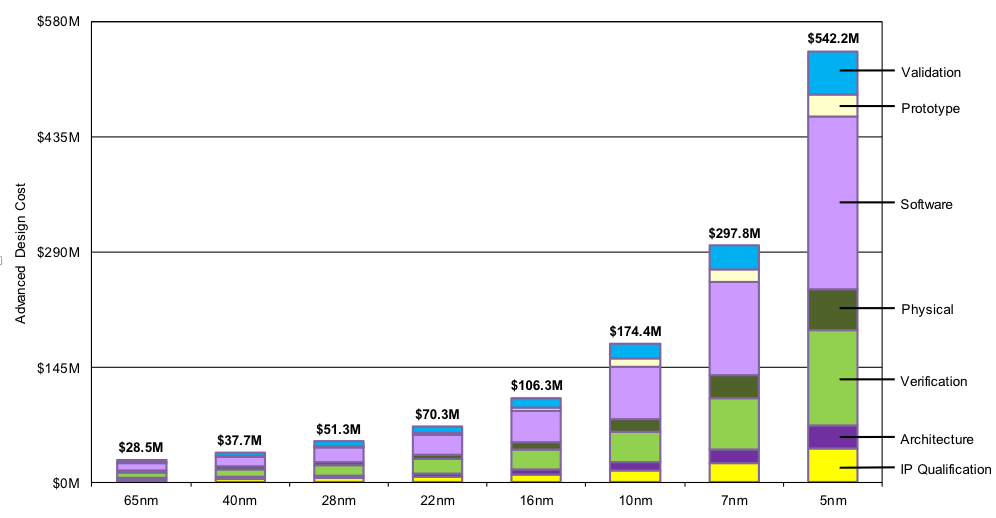
\includegraphics[width=0.99\textwidth]{figures/nre-cost.png}
    \caption{Early design non-recurring engineering~(NRE) cost
    at various feature dimensions. Source: IBS.}
    \label{fig:chip-nre}
\end{figure}

Part of the problem is that there appears to be no silver bullet for reducing
ASIC NRE, as there many disparate sources that often span multiple domains of
chip design~(Figure~\ref{fig:chip-nre}). Instead, we will need many diverse
tooling improvements united under a reimagined methodology for building custom
silicon. At Berkeley, we have articulated one such vision inspired by agile
software-engineering practises~\cite{AgileHW} and have built tools to support it.
These tools include Chisel~\cite{Chisel}, a more productive hardware-design
language (HDL) based in Scala, and FIRRTL~\cite{FIRRTL}, a flexible
intermediate representation for hardware that makes it easier to build
compilers. Perhaps the largest contribution to this vision has been the RISC-V
instruction set architecture~(ISA)~\cite{WatermanDissertation}.  Being open and
free-to-use, RISC-V enables chip designers to build customized microprocessors
while extending an open-source software toolchain.  This avoids the costs and
legal encumbarances of using a priopreitary ISA, or the massive engineering
burden of developing a fully custom ISA. RISC-V adoption has been meteoric in
recent years, both in academia outside of Berkeley~\cite{BlackParrot, Celerity,
Pulp}, and in industry, where a growing body of companies, notably SiFive,
Western Digital, and Nvidia have been developing new RISC-V implementations.

One unaddressed deficiency in chip design that drives verification, validation and software development
costs, is the lack of a good full-system simulation technology. Ideally, such
a technology would be:
\begin{itemize}
    \item \textbf{Fast.} As fast as silicon prototype, so as to enable running full system
    stacks and complete applications.
\item \textbf{Detailed.} It would simulate SoC's timing characteristics exactly.
\item \textbf{Productive.} It would be easy to debug and fast to recompile.  It would feel much like a software-based simulator.
\item \textbf{Inexpensive.} It would be cheap to deploy so that it could be made widely accessible
        to hardware and software design teams and support running large parallel experiments.
\end{itemize}

In practise, existing simulation technologies are forced to prioritize two of
these objectives. Software simulators, despite being easy to use and relatively
inexpensive, are much too slow to run full-system simulations when providing a
cycle-accurate model of the chip. For speed, chip designers are forced to turn
to hardware acceleration, in the form of FPGA prototyping and hardware
emulation.  Of the two, FPGA prototypes tend to be faster and less expensive,
and so see extensive use in software development and regression testing later
in the design cycle.  Conversely, hardware emulation is slower and considerably
more expensive, but offers a software-simulator-like debugging experience that
makes it a critical tool for pre-silicon verification. We will expand more on these
differences in Chapter~\ref{sec:simulation-background}.

The central question of the simulation work underway at Berkeley asks if it is
possible to build a simulation platform that can marry the speed of FPGA
prototyping, and the productivity of hardware emulation, while being radically
cheaper to deploy. Such a technology would put hardware emulation in the hands
of smaller research groups, and make it more widely available in companies
where scarse emulation resources must be carefully scheduled. Additionally, if
it is fast enough, it could subsume the role of a conventional FPGA prototype,
reducing the engineering burden of having parallel emulation and FPGA
prototyping infrastructures. If this technology is going to be inexpensive, two
things are clear.  First, it must use commericial off-the-shelf~(COTS) FPGA
platforms, and not custom devices or system integration as is true of all
commerical emulators. Second, this technology's software ecosystem, including
tools and IP libraries, will need to be open-source with the hope that they can
be developed and maintained by a community of users instead of a private team
of engineers.

This is no small undertaking but one made easier by recent technology trends.
Firstly, modern FPGAs are enormous, continue to be amoung the greatest
beneficiaries of Moore's law since they can naturally scale to use larger
transistor budgets. Advances in multi-die integration technologies have made
it easier to reliably manufacture even larger FPGAs. This makes it possible to
simulate considerably larger systems on a single FPGA.  Secondly, FPGAs are now available
in public cloud and provided by many major vendors like Amazon Web Services~\cite{amazonf1}.
This means a team can avoid the expense of building and
maintaining their own local FPGA cluster, and can use newer FPGAs as they
become available. Cloud services also provide an elastic supply of FPGAs,
allowing users to scale out experiments as needed, instead of needing to
provision a local cluster for the worst case. While the rates of using
cloud-based FPGAs are currently non-trivial, we expect these to fall in the
future as the costs of these services are amortized. Finally, it would be
difficult to build out an emulation infrastucture without the aforementioned advances in
open-source tooling. A compiler lies at the heart of all hardware emulation systems:
FIRRTL and its and Scala-based compiler infrastructure provide flexible
abstractions for translating a design into an FPGA-hosted emulator. FPGA-hosted emulation
infrastucture requires customized hardware, and more productive hardware-design
languages, like Chisel, makes it considerably easier for a small team to build
it. Finally, for an open-source infrastructure to see use, it
requires open-source input designs to both encourage adoption and inform
development. Here, we can leverage a growing body of RISC-V based processors,
such as Rocket~\cite{RocketChip} and BOOM~\cite{BOOM}, to feed into our system.

While it initially began as a project to study warehouse-scale computers, the
FireSim~\cite{FireSim} project has been our attempt at building out this
new technology. FireSim has been the basis for a
number of emulation-related research papers at Berkeley: we have studied
detailed DRAM timing models~\cite{FASED}, non-invasive, full-system profiling
techniques~\cite{FirePerf}.  FireSim-adjacent projects, using the same
underlying compiler, MIDAS~\cite{MIDAS}, have explored novel techniques for rapid
debugging~\cite{DESSERT}, and energy estimation~\cite{Simmani, Strober}. Over
time, features from these projects have gradually been integrated in mainline
FireSim, where they are employed by a growing user base.

Unfortunately, limitations with MIDAS limited its scope
to simple designs. First, these designs were small: they could be directly
implemented on a single Xilinx Ultrascale+ VU9P FPGA. In contrast, FPGA prototypes
of modern SoCs require partitioning over multiple FPGAs~\cite{FPMM}.  Second, these systems possessed only a single
clock domain. Conversly, modern SoCs have dozens of clocks whose frequencies
may change during execution. Without the ability to simulate
even a small number of fixed-frequency clocks it was difficult to get truly
accurate performance estimates with FireSim. Addressing these two challenges
drove the design of a new optimizing-compiler called Golden Gate~\cite{GoldenGate}.

To simulate larger systems, Golden Gate uses multi-cycle resource optimizations
to replace FPGA-hostile blocks. Golden Gate automates many techniques
deployed in prior academic work in FPGA-accelerated microarchitecture
simulation to radically improve the capacity of single FPGA. These
optimizations are the focus of Albert Magyar's dissertation~\cite{MagyarDissertation}.
Addressing the second challenge of simulating systems with more realistic clock
organizations is the subject of this dissertation. The contribution of this
work are threefold:

\begin{enumerate}
\item We describe Golden Gate, an optimizing compiler infratructure to deploy module-based
    multi-cycle resource optimizations~(Chapter~\ref{sec:golden-gate}. This
    contribution is shared with Albert Magyar, and is also described in his
    dissertation.

\item A simple, FPGA-flexible, extension to Golden Gate to support systems
    with fixed frequency clocks that is compatible with multi-cycle resource optimizations~(Chapter~\ref{sec:static-multiclock}).

\item A general, distributed approach for simulating clock generating and switching structures,
    based off of  prior work in software parallel discrete-event
    simulation~(Chapter~\ref{sec:dynamic-multiclock}). As above, our
    implementation co-exists with all multi-cycle resource
    optimizations.
\end{enumerate}

All of the software described in this dissertation is open source. We make
frequent reference to specific versions of the FireSim codebase to provide more
context in each chapter. Code references will use \texttt{monospace typeface}
where applicable. We hope this will help document features of FireSim as more
users adopt it. At time of writing, Golden Gate and support for fixed-frequency
clocks~(Chapter~\ref{sec:static-multiclock}) have been integrated into mainline
FireSim and are under active use. The features described in
Chapter~\ref{sec:dynamic-multiclock} are tagged \texttt{pdes}, and will be
merged in the future.

\section{Previous Publication, Collaboration, and Funding}

Portions of this work were published at the 2019 International Conference on
Computer-Aided Design as ``Golden Gate: Bridging The Resource-Efficiency Gap
Between ASICs and FPGA Prototypes'', though in this dissertation we focus on
the design of the compiler. The specific resource optimization employed in that
publication is described at length in Albert Magyar's dissertation~\cite{MagyarDissertation}.  Early results
from our initial support for emulation of multiple fixed-frequency
phase-aligned clocks, were published as ``Accessible, Resource-Efficient
FPGA-Accelerated Emulation Using FireSim'' in a July 2021 IEEE MICRO special
issue on FPGAs in Computing.

Donggyu Kim drove the bulk of MIDAS development based on his work on
Strober~\cite{Strober}. In the ``1.0" version of MIDAS presented in his
dissertation~\cite{DGKDissertation}, I contributed the design of endpoint
system. The final version of that compiler used by FireSim is described in
Chapter~\ref{sec:fpga-des}.

The work uses features developed by other FireSim contributors. Notable
contributors include Alon Amid, who developed much of the debug infrastructure,
Howard Mao, who has contributed to nearly all subsystems in FireSim, and Sagar
Karandikar, who ported MIDAS to use AWS and designed the cloud manager.

Finally, Golden Gate was the product of a tight collaboration between myself
and Albert Magyar. Much of the complexity in our dissertations is tied to the
FIRRTL-based software instructure required to analyze target SoCs and transform
them into latency-insensitive networks. This common infrastructure is described
at length in Chapter~\ref{sec:golden-gate}, and is the basis for the remainder
of the disseration.

The information, data, or work presented herein was funded in part by the
Advanced Research Projects Agency-Energy (ARPA-E), U.S. Department of Energy,
under Award Number DE-AR0000849.  Research was partially funded by ADEPT Lab
industrial sponsors and affiliates Intel, Apple, Futurewei, Google, and
Seagate.  The views and opinions of authors expressed herein do not necessarily
state or reflect those of the United States Government or any agency thereof.

